\documentclass[letterpaper,10pt]{article}

\usepackage{titling}
\usepackage{listings}
\usepackage{url}
\usepackage{setspace}
\usepackage{subfig}
\usepackage{sectsty}
\usepackage{pdfpages}
\usepackage{colortbl}
\usepackage{multirow}
\usepackage{relsize}
\usepackage{amsmath}
\usepackage{fancyvrb}
\usepackage{amsmath,amssymb,amsthm,graphicx,xspace}
\usepackage[titlenotnumbered,noend,noline]{algorithm2e}
\usepackage[compact]{titlesec}
\usepackage[default]{droidserif}
\usepackage[T1]{fontenc}
\usepackage{tikz}
\usetikzlibrary{arrows,automata,shapes,trees,matrix,chains,scopes,positioning,calc}
\tikzstyle{block} = [rectangle, draw, fill=blue!20, 
    text width=2.5em, text centered, rounded corners, minimum height=2em]
\tikzstyle{bw} = [rectangle, draw, fill=blue!20, 
    text width=4em, text centered, rounded corners, minimum height=2em]

\definecolor{namerow}{cmyk}{.40,.40,.40,.40}
\definecolor{namecol}{cmyk}{.40,.40,.40,.40}

\let\LaTeXtitle\title
\renewcommand{\title}[1]{\LaTeXtitle{\textsf{#1}}}


\newcommand{\handout}[5]{
  \noindent
  \begin{center}
  \framebox{
    \vbox{
      \hbox to 5.78in { {\bf ECE155: Engineering Design with Embedded Systems } \hfill #2 }
      \vspace{4mm}
      \hbox to 5.78in { {\Large \hfill #4  \hfill} }
      \vspace{2mm}
      \hbox to 5.78in { {\em #3 \hfill} }
    }
  }
  \end{center}
  \vspace*{4mm}
}

\newcommand{\lecture}[3]{\handout{#1}{#2}{#3}{Lecture #1}}
\newcommand{\tuple}[1]{\ensuremath{\left\langle #1 \right\rangle}\xspace}

\addtolength{\oddsidemargin}{-1.000in}
\addtolength{\evensidemargin}{-0.500in}
\addtolength{\textwidth}{2.0in}
\addtolength{\topmargin}{-1.000in}
\addtolength{\textheight}{1.75in}
\addtolength{\parskip}{\baselineskip}
\setlength{\parindent}{0in}
\renewcommand{\baselinestretch}{1.5}
\newcommand{\term}{Spring 2014}

\singlespace


\begin{document}

\lecture{ 5 --- XML, Android \& Eclipse}{\term}{Jeff Zarnett, based on original by Patrick Lam}

\section*{XML}
You need to know a bit about
XML (e\textbf{X}tensible \textbf{M}arkup \textbf{L}anguage)  to build Android applications, so here's a quick description.  By
the way, this is examinable material.

For further reading, you can consult many resources on the Web.
Here's one:
\begin{center}
\url{http://www.w3schools.com/xml/default.asp}
\end{center}

\paragraph{XML in one line.}
\begin{center}
XML is a \emph{structured document format}.
\end{center}

All XML documents therefore have the same format. However, XML
has no intrinsic meaning. It just separates content from structure, and to be human readable. If you are familiar with HTML, there are a number of similarities, except where HTML (HyperText Markup Language) is specific to drawing web pages, XML is intended to be general and human-readable.

Every XML document begins with \verb+<?xml version="1.0" encoding="utf-8"?>+, declaring that the document is XML. After that it has \emph{tags}, which are elements of the XML document and appear between angle brackets like \texttt{<example>}. Tags are opened and closed, so that tag must be followed by \texttt{</example>}, which closes the \texttt{example} tag. We can also have ``self-closing'' tabs, a notational convenience where a tag is opened and closed all at once, such as \texttt{<approval/>} (the slash at the end indicates self-closing). A tag may also have attributes, like colour in this example: \texttt{<square colour=``red''/>}.

XML is intended to be human-readable and human writeable. Computers can read and comprehend XML by ``parsing'' the document. There are a number of well-known and well-developed XML parsers; use one of them if you need to programmatically examine some XML and do not write your own.

Let's look at an example of an Android manifest. It's an XML format
document.



\newpage

{\scriptsize
\def\rootnode{\tikz[remember picture] \node[yshift=-.8em] (root) {};}  
\def\attributenode{\tikz[remember picture] \node[yshift=-.8em] (attribute) {};}  
\def\mustQuote{\tikz[remember picture] \node[yshift=-.8em] (mustQuote) {};}  
\def\selfclosing{\tikz[remember picture] \node[yshift=-.8em] (selfclosing) {};}  
\def\nested{\tikz[remember picture] \node[yshift=-.8em] (nested) {};}  
\def\morenested{\tikz[remember picture] \node[yshift=-.8em] (moreNested) {};}  

\begin{Verbatim} [commandchars=\|\-\! ]
<?xml version="1.0" encoding="utf-8"?>
<manifest |rootnode
  xmlns:android="http://schemas.android.com/apk/res/android"
  package="ca.uwaterloo.Lab1_plam"  |attributenode
  android:versionCode="1" |mustQuote
  android:versionName="1.0" >

  <uses-sdk
    android:minSdkVersion="10"
    android:targetSdkVersion="16" /> |selfclosing

  <application |nested
    android:allowBackup="true"
    android:icon="@drawable/ic_launcher"
    android:label="@string/app_name"
    android:theme="@style/AppTheme" >
    <activity |morenested
      android:name="ca.uwaterloo.Lab1_plam.MainActivity"
      android:label="@string/app_name" >
      <intent-filter>
          <action android:name="android.intent.action.MAIN" />
          <category android:name="android.intent.category.LAUNCHER" />
      </intent-filter>
    </activity>
  </application>

  <uses-permission android:name="android.permission.READ_CONTACTS" /> 
  <uses-permission android:name="android.permission.WRITE_CONTACTS" />

</manifest>
\end{Verbatim}
\begin{tikzpicture}[remember picture,overlay]
 \node[right of=root,xshift=2em] (rootLabel) {root node};
 \path[->,line width=1pt,>=latex] (root) edge (rootLabel);

 \node[right of=attribute,xshift=12em] (attributeLabel) {attribute, name is ``package'', value is ``\ldots Lab1\_plam''.};
 \path[->,line width=1pt,>=latex] (attribute) edge (attributeLabel);

 \node[right of=selfclosing,xshift=2em] (selfclosingLabel) {self-closing tag};
 \path[->,line width=1pt,>=latex] (selfclosing) edge (selfclosingLabel);

 \node[right of=mustQuote,xshift=11em] (mustQuoteLabel) {must quote all values, e.g. ``1''};
 \path[->,line width=1pt,>=latex] (mustQuote) edge (mustQuoteLabel);

 \node[right of=nested,xshift=9em] (nestedLabel) {{\tt application} tag is nested within {\tt manifest} tag};
 \path[->,line width=1pt,>=latex] (nested) edge (nestedLabel);

 \node[right of=moreNested,xshift=5em] (moreNestedLabel) {more nesting};
 \path[->,line width=1pt,>=latex] (moreNested) edge (moreNestedLabel);

\end{tikzpicture} 

}


\paragraph{Structure of XML files.}
XML is always tree-structured: at the top level, there is a
\emph{root} element. (Ignore the XML declaration.) So we can convert
the textual form above into a tree. Tags must be well-nested:
you can't open a tag \verb+<a>+ and then close a tag \verb+</b>+
without closing \verb+</a>+ first.

\tikzstyle{every node}=[draw=black,thick,anchor=west,text width=7em]

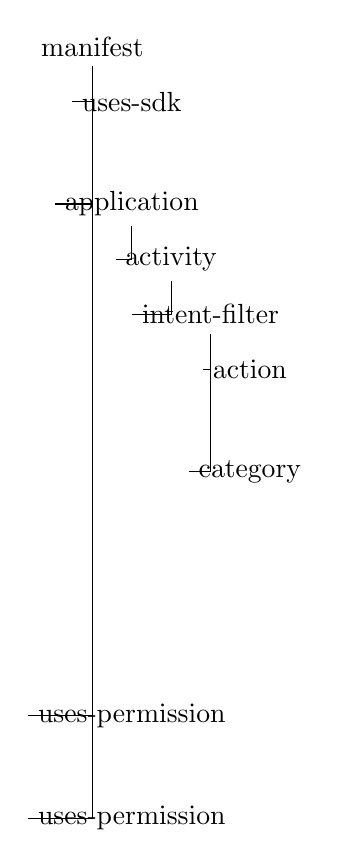
\begin{tikzpicture}[%
  grow via three points={one child at (0.5,-0.7) and
  two children at (0.5,-0.7) and (0.5,-2.0)},
  edge from parent path={(\tikzparentnode.south) |- (\tikzchildnode.west)}]
  \node {manifest}
    child { node {uses-sdk} }		
    child { node {application} child { node {activity} child { node {intent-filter} child { node {action}} child { node {category} } } } }
    child [missing] {}
    child [missing] {}
    child [missing] {}
    child [missing] {}
    child { node {uses-permission} }
    child { node {uses-permission} };
\end{tikzpicture}


\section*{Android}
By now you have no doubt taken a look at the labs and seen that you need to implement them using Android, either on your own phone or one of the devices we provide in the labs. We will take some time to introduce you to Android programming.

\subsection*{Android Activity class}
\begin{center}
``An activity is a single, focused thing that the user can do.''
\end{center}

Usually, an Activity corresponds to a full-screen window which 
the user may interact with. For instance, the user may:
\begin{itemize}
\item set up a timer; 
\item read off sensor values; or
\item make a phone call.
\end{itemize}

Applications may contain multiple activities, each of which
corresponds to a thing that the user wants to do.  Android organizes
activities into tasks.  A task consists of a last-in, first-out stack
of activities, possibly from different applications.

\paragraph{Task Navigation: the Back button.}
The Back button pops the topmost activity off the stack and
gets rid of it.

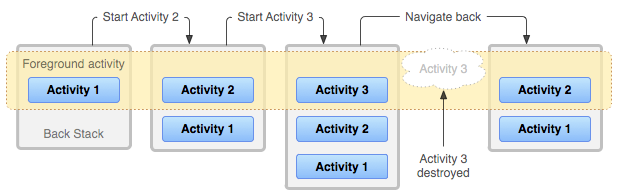
\includegraphics[width=\textwidth]{images/diagram_backstack}\cite{android:backstack}

\paragraph{Task Navigation: switching tasks.} 
It is also possible to switch between tasks.
Switching tasks puts a different activity and its stack
in the foreground, and puts the old activity in the background.

\begin{center}
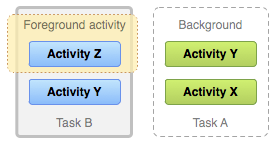
\includegraphics[width=.5\textwidth]{images/diagram_multitasking}\cite{android:multitasking}
\end{center}


\subsection*{Doing Something in Your Activity}
The most useful activity method, where you'll be writing a lot of
code, is \texttt{onCreate()}. It gets executed when the activity 
starts. Typically, it will set up the user interface, namely:
\begin{itemize}
\item creating widgets;
\item setting up event listeners;
\end{itemize}

Note that you must call {\texttt{\textbf{super.onCreate()}}}; this
is taken care of for you in the autogenerated boilerplate code.

\paragraph{Retrieving Widgets} If you've declared widgets in the
XML file, you can use the {\texttt{\textbf{findViewById()}}} method
to get a hold of them. Note:
\begin{itemize}
\item you need to cast the return value, e.g. \\
\texttt{\textbf{tv = (TextView) findViewById(R.id.t);}}
\item you must save the XML file to get the right ids on the {\tt R} object.
\end{itemize}

\paragraph{Programmatically Adding Widgets} We ask you to
add widgets programmatically in Lab 1. There are two steps:
\begin{enumerate}
\item Create the widget: 
\texttt{\textbf{~tv = new TextView(getApplicationContext());}} 
\item Add it to the Activity:
\texttt{\textbf{~addView(tv);}}
\end{enumerate}

\subsection*{Activity Lifecycle}
Although we've only talked about {\tt onCreate()}, there are numerous
other methods on {\tt Activity} which Android calls at various times
(inversion of control!)

\begin{center}
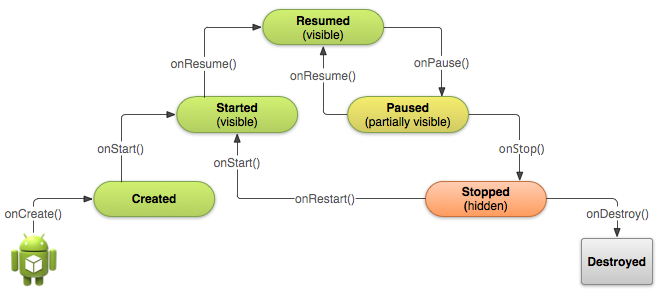
\includegraphics[width=.9\textwidth]{images/basic-lifecycle}\cite{android:lifecycle}
\end{center}


\section*{Integrated Development Environments}

We've seen a bit now about the basics of Android, but let's take a few moments to look at the tools used to work with Android.

\subsection*{In the Dark Ages}
In the dark ages we used to write our code in an editor (\texttt{vi}, \texttt{emacs}, \texttt{notepad.exe}), then call the command line compiler. Actually, sometimes in later courses, you're still going to do this. When writing code in a plain text editor, it just looks like text. Then when you go to compile your code, the compiler prints out a whole pile of errors and you have to sort through and figure out what they all mean.

Then some clever people came up with an idea: what if we changed the tools to make it easier to write and make it less likely people will make a mistake? Hence, integrated development environments. 


\subsection*{Modern IDEs}
IDEs combine a number of tools in a single environment to improve
programmer productivity. These tools include an editor, a compiler,
and a debugger. The IDE concept has been around for over 25 years.

By now you have worked with Eclipse in the labs and presumably you used Microsoft Visual Studio when programming in C\# for ECE~150. Eclipse is free software: you can download the code and modify it yourself. Also, it was initially developed by IBM in Ottawa.

Beyond the three core tools, IDEs can also contain support for
collaboration (revision control systems, which we'll discuss);
documentation and modelling, e.g. UML diagrams; and extensible
programmer tools like autocomplete and refactoring. I'll talk a bit
about autocomplete today.

Let's examine, however, some features of IDEs and how they make programming easier.

\paragraph{Syntax Highlighting} The IDE highlights different syntax of the program, by making them different colours. It makes it easier to see and understand different parts of the code, and makes it possible to detect errors. For example, if you forgot a '' (close-quote) character at the end of a string, then subsequent code after where you expect will be string-coloured, revealing the error. Similarly, comments are often coloured so you can see at a glance if half a line is commented out.


\paragraph{Templates.} IDEs often allow you to start your
project from a template, which is easier than starting from scratch.
You've used the Android Application Project template. Some other
useful templates:
\begin{itemize}
\item Android Test Project (you'll use these);
\item Java Project
\item Java Class
\item Java Interface
\end{itemize}

\paragraph{Project Development Workflow.}
I'll just recap the steps here.

\begin{enumerate}
\setcounter{enumi}{-1}\setlength{\itemsep}{-.5em}
\item Figure out what you'll need to do.
\item Start a new project from a template or, more realistically,
  check it out from a version control repository.
\item Make the edits that you need. 
\item Test your edits by running the application.
\item Debug your edits.
\item Commit your files to the version control repository.
\end{enumerate}

\paragraph{Content Assist.} Even if you type really fast,
Eclipse can help you enter code more quickly, with the Content Assist helper.
Start typing a name and hit Ctrl-Space (still ctrl-space if you're a Mac user). Eclipse will give you a
choice of names to choose from, and you can choose the correct one.
For further reading, see:
\begin{center}\small
\url{http://wiki.eclipse.org/FAQ_How_can_Content_Assist_make_me_the_fastest_coder_ever%3F}
\end{center}
Content Assist can also help you with filling in templates.
You can type ``for'' into Eclipse, hit Ctrl-Space, and choose the 
type of for loop you're trying to write. Choosing ``for --- iterate over array''
inserts the template:
\begin{verbatim}
    for (int i = 0; i < array.length; i++) {

    }
\end{verbatim}
and puts your cursor at the ``i'' so that you can choose your own
index variable. Of course, you still have to figure out what your
code needs to do.

\paragraph{Continuous Compiling} Instead of manually invoking the compiler manually, modern IDEs are constantly running the compiler when a file is changed. So as you're working, you'll see errors and warnings right away.

When you get a red (or yellow) squiggle underneath your code (see the figure below) there's an error (or warning). Eclipse and other very clever IDEs can sometimes suggest a solution, in a feature known as...

\paragraph{Quick Fix.} The other really useful Eclipse feature is Quick Fix.

If the squiggle's corresponding editor marker bar (on the left) contains
a lightbulb, you can Quick Fix it. 

\begin{center}
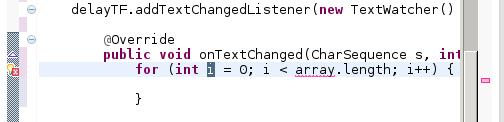
\includegraphics[height=8em]{images/quickfix}
\end{center}

Put the cursor at or near the squiggle, hit Ctrl-1, and Eclipse will
propose some fixes. They may be correct (or not).

You can read more about Quick Fixes in the Eclipse help:
\begin{center}
 Help \textgreater Help Contents \textgreater Java Development User Guide \textgreater Concepts \textgreater Quick Fix
\end{center}


\paragraph{Debugging} 

You may have noticed that sometimes software doesn't quite do what you
want it to do. We call this a \emph{bug}.  We'll discuss some content
from~\cite{zeller09:_why_progr_fail} (highly recommended), in particular
ways to remove bugs from programs.

Three things have to happen before you can observe a bug:\\[-2em]
\begin{enumerate} \setlength{\itemsep}{-.5em} 
\item A programmer puts a defect in the code---some code doesn't do
  what it's supposed to do.
\item This defect sets some program state (e.g. a variable) to an
  incorrect, or ``infected'' value.
\item The infected value has to propagate to program output to cause
an observable failure.
\end{enumerate}

Here is a high-level overview of the debugging process.\\[-2em]
\begin{itemize}
\item Identify the bug and steps to reproduce it.
\item Figure out the cause of the bug.
\item Correct the bug.
\end{itemize}

Eclipse and other IDEs also have tools to help you find out what's going on in your program to help you find a bug. Probably at this point you've already used some of them in the labs (or even in ECE 150!). As an example, it's possible to pause the execution of your software, sometimes, and take a look at the variables while you have it paused.

Soon, we'll have a number of lectures on the subject of debugging, and
explain some techniques (tactics) to help diagnose and fix
problems. Eclipse can help, but the real action is inside your head.





\bibliographystyle{alpha}
\bibliography{155}


\end{document}